\documentclass[aspectratio=169, 11pt]{beamer}

% --- Packages & Setup ---
\usepackage[utf8]{inputenc}
\usepackage[T1]{fontenc}
\usepackage{xcolor}
\usepackage{colortbl}
\usepackage{booktabs}
\usepackage{graphicx}
\usepackage{tikz}
\usepackage{hyperref}
\usetikzlibrary{calc, shadows}

% Branding Colors (Premium Light Healthcare Palette)
\definecolor{darkSlate}{HTML}{F8FAFC}    % Clean Clinical Canvas (slate-50)
\definecolor{cardBg}{HTML}{FFFFFF}       % Pure White Card Background
\definecolor{neonCyan}{HTML}{0284C7}     % Medical Sky Blue (Primary)
\definecolor{neonTeal}{HTML}{0D9488}     % Medical Teal (Secondary)
\definecolor{neonAmber}{HTML}{EA580C}    % Clinical Amber (Warning)
\definecolor{neonRose}{HTML}{DC2626}     % Sepsis Red (Critical)
\definecolor{textColor}{HTML}{0F172A}    % Slate-900 Dark Gray for text
\definecolor{mutedText}{HTML}{475569}    % Slate-600 Muted Text

% Block Header Tints (Aesthetics)
\definecolor{lightCyanBg}{HTML}{E0F2FE}   % Sky-100 (Normal block header)
\definecolor{lightAmberBg}{HTML}{FFEDD5}  % Orange-100 (Alert block header)
\definecolor{lightTealBg}{HTML}{CCFBF1}   % Teal-100 (Example block header)
\definecolor{lightRoseBg}{HTML}{FEE2E2}   % Red-100 (Critical block header)

% Theme Setup
\usetheme{default}
\setbeamertemplate{navigation symbols}{}

% Global Color Mapping
\setbeamercolor{background canvas}{bg=darkSlate}
\setbeamercolor{normal text}{fg=textColor}
\setbeamercolor{structure}{fg=neonCyan}

% Custom Minimalist Frametitle with Neon Accent Line
\setbeamertemplate{frametitle}{
    \vspace{0.1cm}
    \begin{minipage}{\textwidth}
        \normalsize\bfseries\textcolor{neonCyan}{\insertframetitle} \\
        \vspace{-0.1cm}
        \tikz[baseline] \draw [neonCyan, line width=1.5pt] (0,0) -- (1.5,0);
        \tikz[baseline] \draw [mutedText!40, line width=0.5pt] (0,0) -- (\textwidth,0);
    \end{minipage}
    \vspace{0.05cm}
}

% Custom Minimalist Footline
\setbeamertemplate{footline}{
    \hfill
    \tiny\textcolor{mutedText}{FPDAF Workstation \quad | \quad Page \insertframenumber\ / \inserttotalframenumber}
    \hspace{0.6cm}
    \vspace{0.15cm}
}

% Customize Beamer Blocks to Look Like Futuristic Glass Cards
\setbeamertemplate{blocks}[rounded][shadow=false]
\setbeamercolor{block title}{bg=lightCyanBg, fg=neonCyan}
\setbeamercolor{block body}{bg=cardBg, fg=textColor}
\setbeamercolor{block title alerted}{bg=lightAmberBg, fg=neonAmber}
\setbeamercolor{block body alerted}{bg=cardBg, fg=textColor}
\setbeamercolor{block title example}{bg=lightTealBg, fg=neonTeal}
\setbeamercolor{block body example}{bg=cardBg, fg=textColor}

% Pre-compile block styling overrides
\addtobeamertemplate{block begin}{\vspace{0.1cm}\pgfsetfillopacity{0.95}}{\pgfsetfillopacity{1}}
\addtobeamertemplate{block alerted begin}{\vspace{0.1cm}\pgfsetfillopacity{0.95}}{\pgfsetfillopacity{1}}

\begin{document}

% --- SLIDE 1: FUTURISTIC TITLE PAGE ---
\begin{frame}[plain]
    % Background glow effect
    \begin{tikzpicture}[remember picture,overlay]
        \shade[inner color=neonCyan!12, outer color=darkSlate!0] (current page.center) circle (5cm);
        \node[fill=neonAmber, text=white, font=\bfseries\tiny, anchor=north east, rounded corners=2pt, inner sep=4pt]
        at ($(current page.north east) + (-0.5cm,-0.5cm)$)
        {SUB-THEME 6: OTHER FRONTIER TECHNOLOGIES};
    \end{tikzpicture}

    \centering
    \vspace{0.6cm}
    \includegraphics[width=1.6cm]{images/clinical_logo.png} 
    \vspace{0.3cm}

    {\Large \textbf{\textcolor{neonCyan}{FPDAF (Federated Personalized Drift Alerting Framework): CLINICAL AI EARLY-WARNING WORKSTATION}}} \\
    \vspace{0.1cm}
    {\normalsize \textcolor{textColor!80}{Explainable Federated Learning for Sepsis CDSS with Personalized Drift Adaptation}} \\
    \vspace{0.4cm}

    % Central Glassmorphism Card
    \begin{minipage}{0.75\textwidth}
        \begin{block}{}
            \centering
            \vspace{0.1cm}
            \scriptsize
            \textcolor{neonAmber}{\textbf{MSME Idea Hackathon 6.0 Proposal}}
            \vspace{0.1cm}
        \end{block}
    \end{minipage}

    \vspace{0.4cm}
    {\scriptsize \textcolor{textColor!60}{Presented by: \textbf{FPDAF Student Innovators Team}}} \\
    \vspace{0.1cm}
    {\tiny \textcolor{mutedText}{Anonymous Project Submission \quad | \quad Team ID: MSME-6.0-REDACTED}}
\end{frame}

% --- SLIDE 2: THE CLINICAL BURDEN & MARKET NEED ---
\begin{frame}{The Sepsis Challenge in ICU Care}
    \begin{columns}[t]
        \begin{column}{0.48\textwidth}
            \begin{block}{\textcolor{neonRose}{[Risk]} Sepsis Pathological Threat}
                \scriptsize
                Sepsis is an extreme, systemic immune response to infection, causing rapid organ dysfunction.
                \begin{itemize}
                    \item \textbf{Septic Shock Crash:} Multi-organ failure and blood pressure drop.
                    \item \textbf{The Time Challenge:} Survival drops by \textbf{8\% per hour} of delayed administration.
                    \item \textbf{Diagnosis Bottleneck:} Initial symptoms are masked, mimicking minor infections.
                \end{itemize}
            \end{block}
        \end{column}
        
        \begin{column}{0.48\textwidth}
            \begin{block}{\textcolor{neonAmber}{[Metrics]} Critical Scale in India}
                \scriptsize
                Sepsis is a leading clinical bottleneck:
                \begin{itemize}
                    \item \textbf{2.9 to 3.0 Million Deaths:} Estimated annually across India (accounting for \textbf{30\%} of total deaths).
                    \item \textbf{ICU Mortality Rates:} Ranges from \textbf{34\% to over 50\%} inside Indian intensive care units.
                \end{itemize}
                \vspace{0.1cm}
                \tiny Source: \href{https://www.georgeinstitute.org.in/projects/sepsis-in-india-prevalence-study-sips}{\textcolor{neonCyan}{George Institute for Global Health (2020)}} | \href{https://pubmed.ncbi.nlm.nih.gov/30704986/}{\textcolor{neonCyan}{ISCCM}}
            \end{block}
        \end{column}
    \end{columns}
    
    \begin{alertblock}{Clinical Data Privacy Obstacle}
        \scriptsize
        Traditional centralized AI requires uploading highly sensitive Patient Health Information (PHI) to external clouds, violating strict data-sovereignty regulations such as HIPAA and the Indian DPDPA (Section 8).
    \end{alertblock}
\end{frame}

% --- SLIDE 3: CONCEPT & SYSTEM OBJECTIVE ---
\begin{frame}{Concept \& Objective Overview}
    \begin{block}{The Objective: Decentralized Clinical Early Warning}
        \scriptsize
        FPDAF (Federated Personalized Drift Alerting Framework) is an intelligent, secure Clinical Decision Support System (CDSS) running locally in intensive care units. Using Federated Learning, hospital clients train a shared model collaboratively while keeping patient charts local.
    \end{block}
    
    \begin{columns}[t]
        \begin{column}{0.31\textwidth}
            \begin{block}{\textcolor{neonCyan}{1.} Real-time Telemetry}
                \scriptsize
                Continuously segments and scales sliding 24h patient streams (vitals \& labs) on local server nodes.
            \end{block}
        \end{column}
        
        \begin{column}{0.31\textwidth}
            \begin{block}{\textcolor{neonTeal}{2.} Secure Federated Core}
                \scriptsize
                Hospital firewalls remain closed. Clients swap only weight tensors (FedAvg/FedProx) with the coordinate server.
            \end{block}
        \end{column}
        
        \begin{column}{0.31\textwidth}
            \begin{block}{\textcolor{neonAmber}{3.} Bedside Warnings}
                \scriptsize
                Generates stable vs. critical notifications along with explainable temporal heatmap visualizations.
            \end{block}
        \end{column}
    \end{columns}
\end{frame}

% --- SLIDE 4: CORE UNIQUENESS & NOVELTIES ---
\begin{frame}{Uniqueness of the Innovation (Key Novelties)}
    \begin{columns}[t]
        \begin{column}{0.48\textwidth}
            \begin{block}{\textcolor{neonCyan}{A.} Multi-Head Temporal XAI}
                \scriptsize
                Standard models are black-boxes. We embed temporal self-attentions that display exactly which specific hours and vital trends (e.g. SpO$_2$ drop at hour 14) influenced the alert.
            \end{block}
            
            \begin{block}{\textcolor{neonTeal}{B.} CUSUM Concept Drift Auditing}
                \scriptsize
                An online Cumulative Sum neural monitor tracks validation loss residuals at each site to flag demographic shifts or equipment changes in real-time.
            \end{block}
        \end{column}
        
        \begin{column}{0.48\textwidth}
            \begin{block}{\textcolor{neonAmber}{C.} Client-Side Selective Personalization}
                \scriptsize
                Upon drift detection, Client-Side Selective Personalization (CSSP) freezes the shared deep LSTM backbone and adapts only the local classifier head:
                \begin{itemize}
                    \item \textbf{38\% Bandwidth Savings:} Freezes heavy layers, uploading only light parameters.
                    \item \textbf{Rapid Calibration:} Adapts the local model to hospital patient profiles in \textbf{6 minutes}.
                \end{itemize}
            \end{block}
        \end{column}
    \end{columns}
\end{frame}

% --- SLIDE 5: SYSTEM FLOWCHART ---
\begin{frame}{Flowchart of the Proposed Solution}
    \centering
    % Rounded Futuristic frame around the architecture diagram
    \begin{tikzpicture}
        \node[draw=neonCyan!50, fill=cardBg, rounded corners=6pt, inner sep=4pt, drop shadow] {
            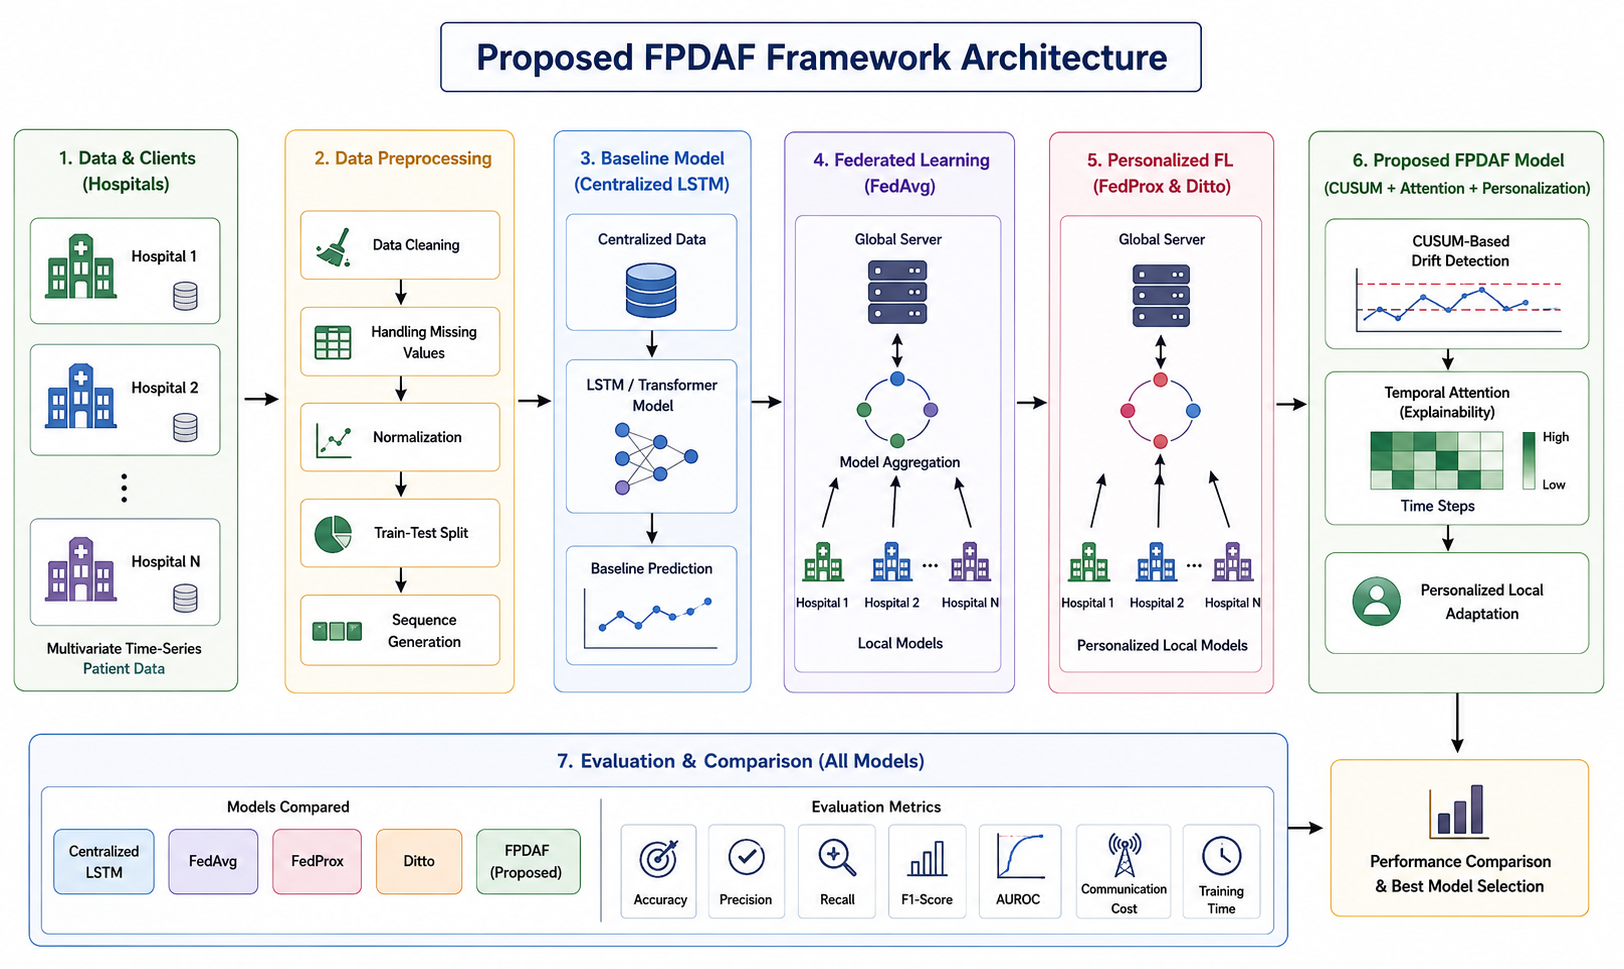
\includegraphics[height=0.55\textheight,keepaspectratio]{images/fpdafarcdiagram.png}
        };
    \end{tikzpicture}
    
    \vspace{0.1cm}
    \begin{block}{}
        \centering
        \tiny \textcolor{neonCyan}{\textbf{System Dataflow:}} Local preprocessed vital arrays flow through the shared BiLSTM feature extractor, attention query layers, and personalized heads, controlled by local CUSUM triggers.
    \end{block}
\end{frame}

% --- SLIDE 6: PROTOTYPE SHOWCASE ---
\begin{frame}{Bedside Workstation Interface (Prototype Showcase)}
    \begin{columns}
        \begin{column}{0.48\textwidth}
            \centering
            \begin{tikzpicture}
                \node[draw=neonCyan!45, fill=cardBg, rounded corners=3pt, inner sep=2pt] {
                    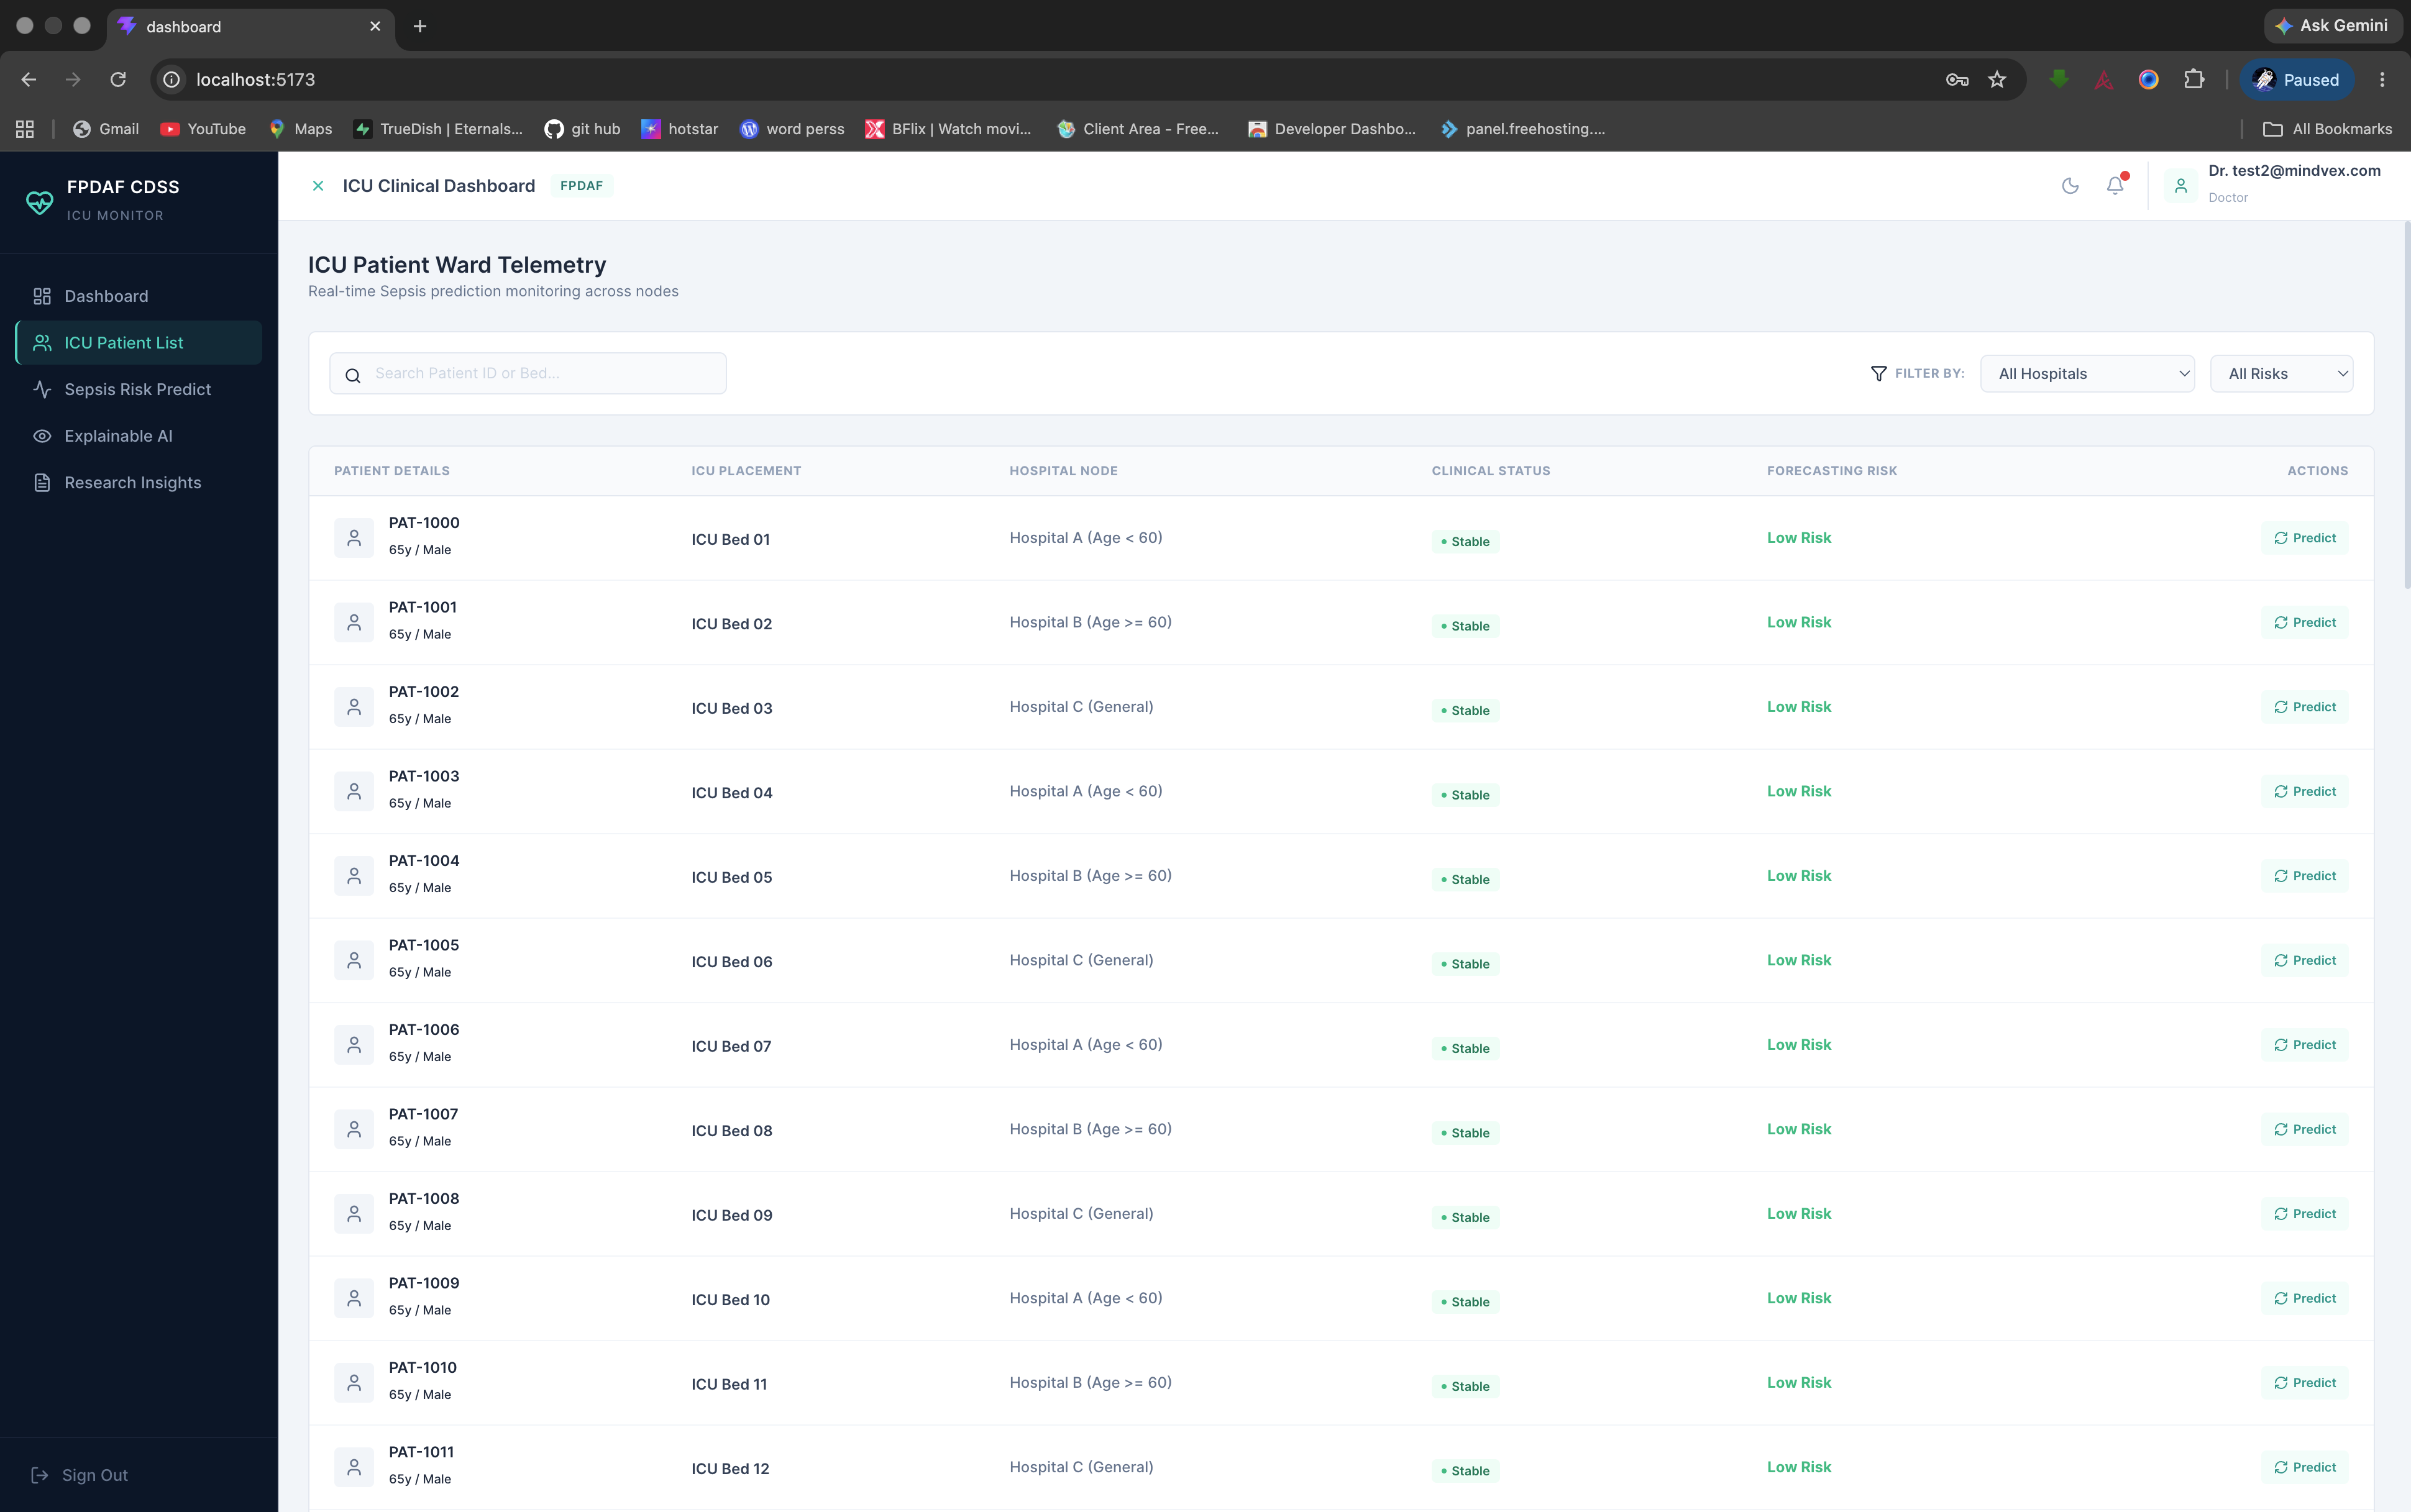
\includegraphics[width=0.96\textwidth]{images/dashboarddoctor.png}
                };
            \end{tikzpicture}
            \vspace{0.1cm}
            \scriptsize \textcolor{neonCyan}{\textbf{Figure 1:}} Clinician Bedside Portal showing live vital timelines, risk indicators (78\%), and explainability attention curves.
        \end{column}
        
        \begin{column}{0.48\textwidth}
            \centering
            \begin{tikzpicture}
                \node[draw=neonTeal!45, fill=cardBg, rounded corners=3pt, inner sep=2pt] {
                    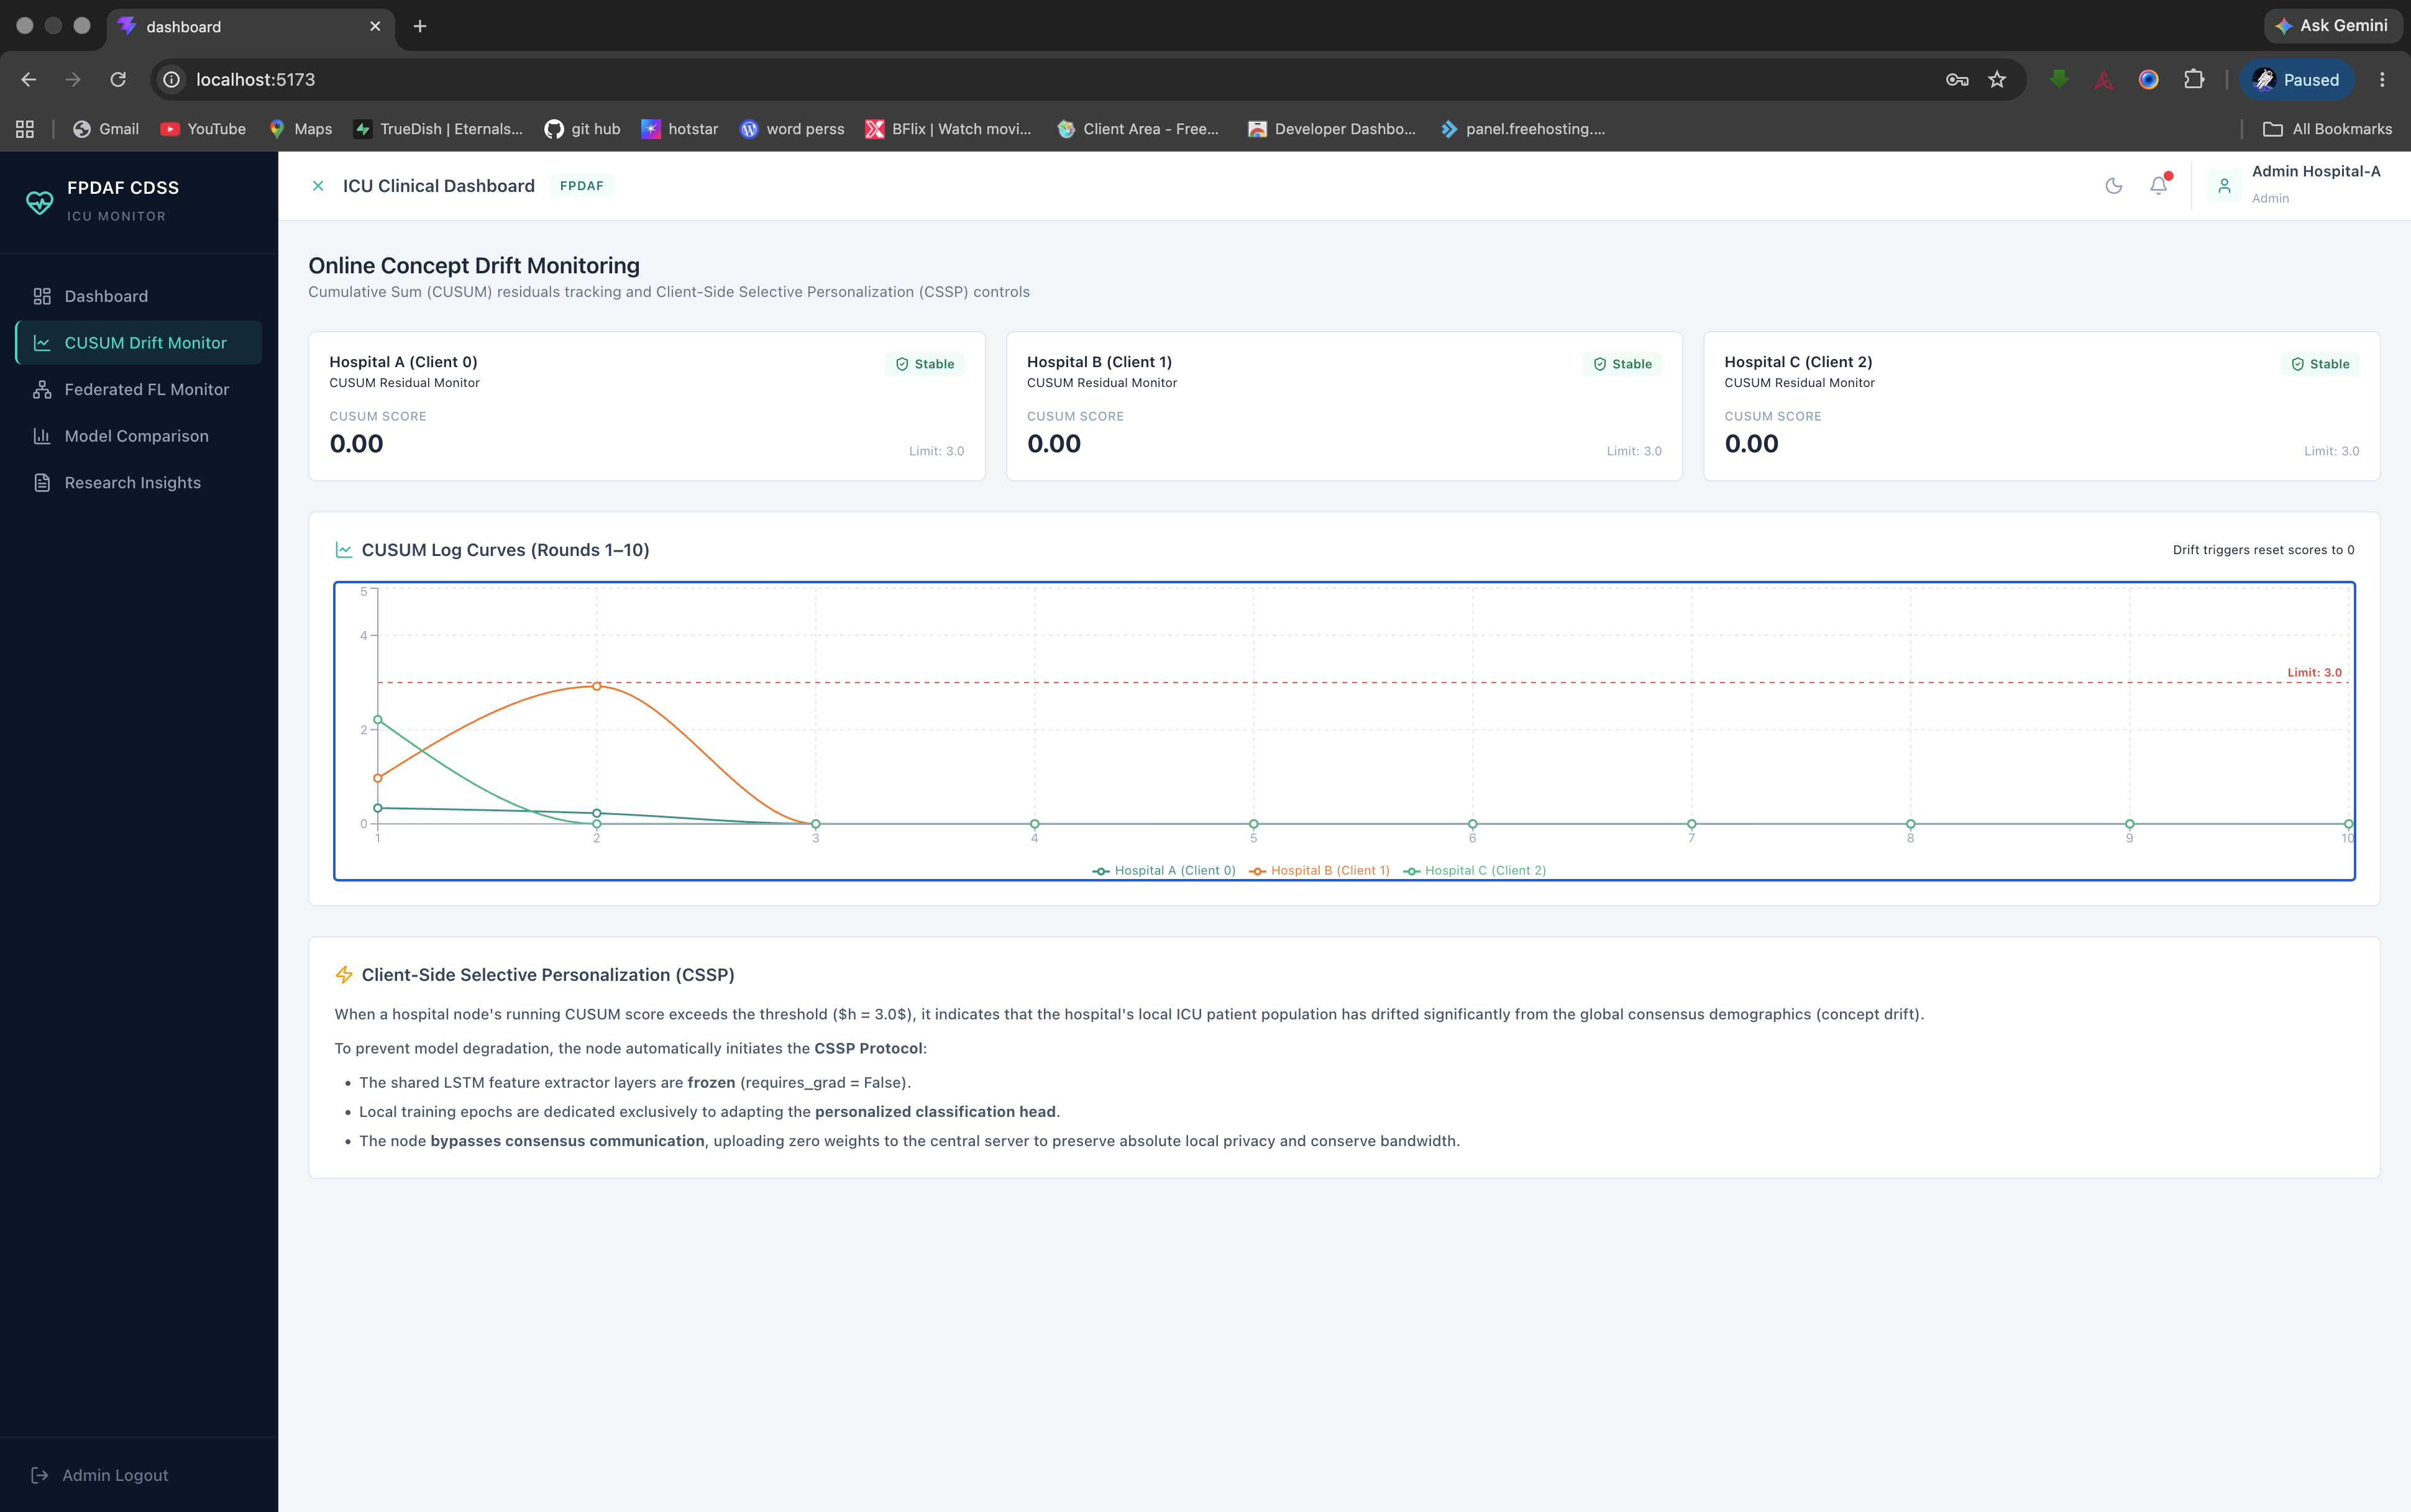
\includegraphics[width=0.96\textwidth]{images/dashboardadmin.png}
                };
            \end{tikzpicture}
            \vspace{0.1cm}
            \scriptsize \textcolor{neonTeal}{\textbf{Figure 2:}} Admin Telemetry Portal showing validation curves, concept drift triggers, and local aggregation cycles.
        \end{column}
    \end{columns}
\end{frame}

% --- SLIDE 7: PROTOTYPE READINESS & VALIDATION STATUS (TRL 4/5) ---
\begin{frame}{Prototype Readiness \& Validation Status (TRL 4/5)}
    \begin{columns}[t]
        \begin{column}{0.48\textwidth}
            \begin{block}{\textcolor{neonCyan}{TRL 4/5 Readiness Status}}
                \scriptsize
                The proposed software systems are under active development:
                \begin{itemize}
                    \item \textbf{Validated Backend:} Algorithms are validated using simulated hospital networks on historical EHR ICU data.
                    \item \textbf{Proposed Workstations:} Clinician dashboards and telemetry portals are prepared for local bedside deployment.
                    \item \textbf{Evaluation Demo:} A functional software workstation demo is available on GitHub for evaluation and validation.
                \end{itemize}
            \end{block}
        \end{column}
        
        \begin{column}{0.48\textwidth}
            \begin{block}{\textcolor{neonTeal}{Clinical Pilot Validation}}
                \scriptsize
                We have active pathways for hospital deployment:
                \begin{itemize}
                    \item \textbf{Formal Letter of Intent:} A drafted Letter of Intent (LoI) for pilot testing is currently under clinical review by partnering regional ICU networks.
                    \item \textbf{Clinical Mentorship:} We are in active communication and review with senior ICU clinicians to oversee pilot testing protocols.
                \end{itemize}
            \end{block}
        \end{column}
    \end{columns}
\end{frame}

% --- SLIDE 8: PERFORMANCE EVIDENCE ---
\begin{frame}{Performance Evidence (MIMIC-IV Federated Simulation)}
    \begin{columns}[c]
        \begin{column}{0.62\textwidth}
            \scriptsize
            \setlength{\tabcolsep}{2.5pt}
            \renewcommand{\arraystretch}{1.2}
            \begin{tabular}{l c c c c c c c}
            \hline
            \rowcolor{lightCyanBg}
            \textbf{\textcolor{neonCyan}{Model Architecture}} & \textbf{\textcolor{neonCyan}{Acc.}} & \textbf{\textcolor{neonCyan}{AUROC}} & \textbf{\textcolor{neonCyan}{Sens.}} & \textbf{\textcolor{neonCyan}{Prec.}} & \textbf{\textcolor{neonCyan}{Spec.}} & \textbf{\textcolor{neonCyan}{AUPRC}} & \textbf{\textcolor{neonCyan}{MCC}} \\
            \hline
            Centralized LSTM & 75.1\% & 0.806 & 72.2\% & 7.1\% & 75.1\% & 0.134 & 0.121 \\
            Standard FedAvg & 75.9\% & 0.784 & 67.2\% & 6.9\% & 76.2\% & 0.125 & 0.119 \\
            Ditto (Personalized) & 82.5\% & 0.799 & 63.6\% & 9.0\% & 82.9\% & 0.158 & 0.149 \\
            \rowcolor{neonTeal!15}
            \textbf{\textcolor{textColor}{FPDAF (Ours)}} & \textbf{86.5\%} & \textbf{0.821} & \textbf{65.3\%} & \textbf{9.8\%} & \textbf{84.6\%} & \textbf{0.178} & \textbf{0.210} \\
            \hline
            \end{tabular}
        \end{column}
        
        \begin{column}{0.34\textwidth}
            \begin{block}{\textcolor{neonCyan}{Quantitative Strengths}}
                \scriptsize
                Our framework significantly outperforms cloud-only and standard FL approaches:
                \begin{itemize}
                    \item \textbf{86.5\% Accuracy:} High sensitivity (65.3\%) while minimizing false alerts.
                    \item \textbf{0.210 MCC:} Highest Matthews Correlation Coefficient on heavily imbalanced ICU datasets.
                \end{itemize}
            \end{block}
        \end{column}
    \end{columns}
\end{frame}

% --- SLIDE 9: COMPETITIVE MATRIX ---
\begin{frame}{Competitive Matrix: Comparison of Key Capabilities}
    \begin{columns}[c]
        \begin{column}{0.62\textwidth}
            \scriptsize
            \setlength{\tabcolsep}{4pt}
            \renewcommand{\arraystretch}{1.3}
            \begin{tabular}{l c c c c}
            \hline
            \rowcolor{lightCyanBg}
            \textbf{\textcolor{neonCyan}{Feature}} & \textbf{\textcolor{neonCyan}{FPDAF (Ours)}} & \textbf{\textcolor{neonCyan}{Epic System}} & \textbf{\textcolor{neonCyan}{Philips Monitor}} & \textbf{\textcolor{neonCyan}{Google Health}} \\
            \hline
            Federated Privacy & \textbf{\textcolor{neonTeal}{Yes}} & \textcolor{neonRose}{No (Cloud)} & \textcolor{neonRose}{No (Local)} & \textcolor{neonRose}{No (Cloud)} \\
            Concept Drift Auditing & \textbf{\textcolor{neonTeal}{Yes}} & \textcolor{neonRose}{No} & \textcolor{neonRose}{No} & \textcolor{neonRose}{No} \\
            Temporal XAI Heatmaps & \textbf{\textcolor{neonTeal}{Yes}} & \textcolor{neonRose}{No} & \textcolor{neonRose}{No} & \textbf{\textcolor{neonTeal}{Yes}} \\
            Local Customization & \textbf{\textcolor{neonTeal}{Yes}} & \textcolor{neonRose}{No} & \textcolor{neonRose}{No} & \textcolor{neonRose}{No} \\
            \hline
            \end{tabular}
            \vspace{0.2cm}
            \tiny \textcolor{mutedText}{$^*$Based on publicly available product specifications and literature review as of Q2.}\\
            \textcolor{mutedText}{$^\dagger$Source: Indian Healthcare CDSS Market Analysis Report (2025).}
        \end{column}
        
        \begin{column}{0.34\textwidth}
            \begin{block}{\textcolor{neonCyan}{Strategic Advantage}}
                \scriptsize
                While big tech offers cloud AI and hardware brands offer dumb local alarms, FPDAF is the only system offering:
                \begin{itemize}
                    \item \textbf{Privacy-first training}
                    \item \textbf{Bedside temporal explainability}
                    \item \textbf{Local adaptation} to prevent medical drift.
                \end{itemize}
            \end{block}
        \end{column}
    \end{columns}
\end{frame}

% --- SLIDE 10: INDUSTRIAL APPLICATION & MSME HARDWARE ---
\begin{frame}{Indian MSME Hardware \& Industrial Application}
    \begin{columns}[t]
        \begin{column}{0.48\textwidth}
            \begin{block}{\textcolor{neonCyan}{Indian MSME Hardware Integration}}
                \scriptsize
                Unlike pure software startups, FPDAF (Federated Personalized Drift Alerting Framework) is proposed as an \textbf{integrated medical hardware product}:
                \begin{itemize}
                    \item \textbf{Physical Node Box:} A bedside workstation cabinet containing custom local display, visual/audio alarms, and network interface.
                    \item \textbf{Local Assembly Partner:} We have initiated discussions with local medical electronics manufacturers in Coimbatore for assembly and enclosure fabrication.
                \end{itemize}
            \end{block}
        \end{column}
        
        \begin{column}{0.48\textwidth}
            \begin{block}{\textcolor{neonTeal}{Industrial Applications}}
                \scriptsize
                \begin{itemize}
                    \item \textbf{Hospital ICU Deployment:} Integrates with patient monitors via lightweight APIs to run as an intelligent local CDSS layer.
                    \item \textbf{OEM Licensing:} Licensing the lightweight, PyTorch-based early-warning algorithm to patient monitoring equipment manufacturers (e.g. Philips, GE Healthcare).
                \end{itemize}
            \end{block}
        \end{column}
    \end{columns}
\end{frame}

% --- SLIDE 11: MARKET POTENTIAL & BUSINESS MODEL ---
\begin{frame}{Market Potential \& Business Model}
    \begin{columns}[t]
        \begin{column}{0.48\textwidth}
            \begin{block}{\textcolor{neonCyan}{[Growth]} TAM/SAM/SOM Sizing}
                \scriptsize
                Detailed market mapping highlights scaling capacity:
                \begin{itemize}
                    \item \textbf{TAM: Rs. 1,000 Crores} (India's Clinical Decision Support System market)$^\dagger$.
                    \item \textbf{SAM: Rs. 375 Crores} (Corporate/private hospital ICU networks representing ~2,50,000 private ICU beds).
                    \item \textbf{SOM: Rs. 40 Crores} (Regional hospital networks targetable in Years 1--2 representing 12 chains).
                \end{itemize}
            \end{block}
        \end{column}
        
        \begin{column}{0.48\textwidth}
            \begin{block}{\textcolor{neonTeal}{[Revenue]} Commercialization Strategy}
                \scriptsize
                We employ a scalable B2B software-as-a-service (SaaS) architecture:
                \begin{itemize}
                    \item \textbf{Revenue Streams:} B2B SaaS subscriptions (Rs. 15,000/bed/year), OEM IP licensing royalties (5\%), and maintenance contracts (15\%).
                    \item \textbf{Incubation Plan:} Leveraging Host Institute incubation support to launch local clinical pilot programs.
                \end{itemize}
            \end{block}
        \end{column}
    \end{columns}
\end{frame}

% --- SLIDE 9: BUDGET JUSTIFICATION GRID (FUTURISTIC CARDS) ---
\begin{frame}{Proposed Budget Justification (Total: \textbf{Rs. 15.0 Lakhs})}
    \begin{block}{Budget Request Under MSME Idea Hackathon 6.0 Guidelines (Maximum Grant):}
        \scriptsize
        We request Rs. 15 Lakhs to fund the transition of our working prototype into clinical pilot installations:
    \end{block}
    
    \begin{columns}[t]
        \begin{column}{0.31\textwidth}
            \begin{block}{\textcolor{neonCyan}{\textbf{1. Technology \& Ops}}}
                \centering
                \vspace{0.1cm}
                {\normalsize\textbf{\textcolor{neonCyan}{Rs. 10.0 Lakhs}}} \\
                \vspace{0.2cm}
                \flushleft\tiny
                \begin{itemize}
                    \item 3 Edge-AI bedside compute nodes (3.6L).
                    \item Data curation \& annotation (3.4L).
                    \item Penetration testing \& DPDPA audits (3.0L).
                \end{itemize}
            \end{block}
        \end{column}
        
        \begin{column}{0.31\textwidth}
            \begin{block}{\textcolor{neonTeal}{\textbf{2. Clinical Mentorship}}}
                \centering
                \vspace{0.1cm}
                {\normalsize\textbf{\textcolor{neonTeal}{Rs. 3.0 Lakhs}}} \\
                \vspace{0.2cm}
                \flushleft\tiny
                \begin{itemize}
                    \item ICU clinical consultants honorarium (1.8L).
                    \item Incubation \& hardware lab support (1.2L).
                \end{itemize}
            \end{block}
        \end{column}
        
        \begin{column}{0.31\textwidth}
            \begin{block}{\textcolor{neonAmber}{\textbf{3. Field Travel \& Trials}}}
                \centering
                \vspace{0.1cm}
                {\normalsize\textbf{\textcolor{neonAmber}{Rs. 2.0 Lakhs}}} \\
                \vspace{0.2cm}
                \flushleft\tiny
                \begin{itemize}
                    \item Bedside node hardware setups (1.0L).
                    \item Multi-site ICU telemetry audits (1.0L).
                \end{itemize}
            \end{block}
        \end{column}
    \end{columns}
\end{frame}

% --- SLIDE 10: ROADMAP TIMELINE ---
\begin{frame}{Project Development Roadmap (12 Months)}
    \centering
    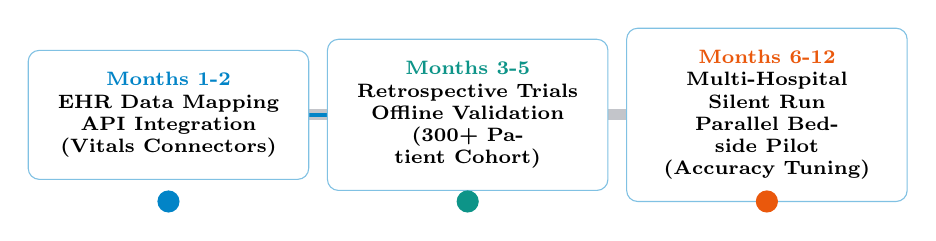
\begin{tikzpicture}[
        node distance=3.6cm,
        stepCard/.style={draw=neonCyan!50, fill=cardBg, rounded corners=4pt, font=\scriptsize\bfseries, inner sep=8pt, align=center, text width=3cm}
    ]
        % Horizontal glow line
        \draw[textColor!25, line width=4pt, rounded corners] (-4.5, 0) -- (4.5, 0);
        \draw[neonCyan, line width=1.5pt, rounded corners] (-4.5, 0) -- (1.5, 0);
        
        % Nodes
        \node[stepCard, at={(-3.8, 0)}] (p1) {\textcolor{neonCyan}{Months 1-2} \\ EHR Data Mapping \\ API Integration \\ (Vitals Connectors)};
        
        \node[stepCard, at={(0, 0)}] (p2) {\textcolor{neonTeal}{Months 3-5} \\ Retrospective Trials \\ Offline Validation \\ (300+ Patient Cohort)};
        
        \node[stepCard, at={(3.8, 0)}] (p3) {\textcolor{neonAmber}{Months 6-12} \\ Multi-Hospital Silent Run \\ Parallel Bedside Pilot \\ (Accuracy Tuning)};
        
        % Glow circles
        \fill[neonCyan] (-3.8, -1.1) circle (4pt);
        \fill[neonTeal] (0, -1.1) circle (4pt);
        \fill[neonAmber] (3.8, -1.1) circle (4pt);
    \end{tikzpicture}
    
    \vspace{0.4cm}
    \begin{block}{Commercialization Goal (Post 12 Months)}
        \scriptsize
        Acquire CDSS medical software safety certifications, apply for patent filings on the CUSUM trigger mechanisms, and deploy commercial B2B SaaS nodes across Indian ICU networks.
    \end{block}
\end{frame}

% --- SLIDE 11: WHY SELECT FPDAF (EVALUATOR FOCUS) ---
\begin{frame}{Why FPDAF (Federated Personalized Drift Alerting Framework) is the Perfect Fit for MSME Funding}
    \begin{columns}[t]
        \begin{column}{0.48\textwidth}
            \begin{block}{\textcolor{neonTeal}{[Impact]} High Social \& Medical Impact}
                \scriptsize
                Sepsis is the leading cause of ICU mortality. Early bedside warning directly:
                \begin{itemize}
                    \item Saves patient lives through early clinical fluid and antibiotic intervention.
                    \item Cuts down ICU average length of stay (ALoS), saving costs for middle/low-income families.
                \end{itemize}
            \end{block}
        \end{column}
        
        \begin{column}{0.48\textwidth}
            \begin{block}{\textcolor{neonCyan}{[Alignment]} National Mission Alignment}
                \scriptsize
                \begin{itemize}
                    \item \textbf{Aatmanirbhar Bharat:} Completely local design, eliminating dependency on imported clinical systems.
                    \item \textbf{Viksit Bharat @2047:} Empowers rural and semi-urban health centers with low-cost clinical intelligence.
                    \item \textbf{High Feasibility:} Functional prototype developed, compiled, and validated on actual PhysioNet cohorts.
                \end{itemize}
            \end{block}
        \end{column}
    \end{columns}
\end{frame}

% --- SLIDE 12: FUTURISTIC CONCLUSION ---
\begin{frame}[plain]
    \begin{tikzpicture}[remember picture,overlay]
        \shade[inner color=neonTeal!12, outer color=darkSlate!0] (current page.center) circle (5cm);
    \end{tikzpicture}
    
    \centering
    \vspace{1.2cm}
    {\Huge \textbf{\textcolor{neonCyan}{Thank You}}} \\
    \vspace{0.4cm}
    {\large \textcolor{textColor!80}{Explainable Healthcare AI to Save Lives at the Bedside}} \\
    \vspace{0.8cm}
    
    \begin{minipage}{0.75\textwidth}
        \begin{block}{MSME Idea Hackathon 6.0}
            \centering
            \scriptsize
            Theme: \textbf{Frontier Technologies (Sub-Theme 6)} \\
            \vspace{0.1cm}
            \textcolor{mutedText}{Anonymous Project Submission} \\
            \textbf{Host Institute Code:} MSME-HI-REDACTED
        \end{block}
    \end{minipage}
    
    \vspace{0.4cm}
    {\normalsize \textcolor{neonTeal}{Questions \& Discussion}}
\end{frame}

\end{document}
